%@TheDoctorRAB
%standard white paper/preproposal format
%
%%%%%
%
%REFERENCES
%
%neup.bst - numbered citations in order of appearance, short author list with et al in reference section
%nsf.bst - numbered citations in order of appearance, full author list in references section
%standard.bst - citations with author last name with et al for more than 2 authors; full author list in references section
%ans.bst is for ANS only. 
%
%author = {Lastname, Firstname and Lastname, Firstname and Lastname, Firstname} for all bst formats
%bst renders the author list itself
%
%author = {{Nuclear Regulatory Commission}} if the author is an organization, institution, etc., and not people
%
%title = {{}} for all
%
%for all - use \citep{-} - [1] or (Borrelli, 2021) in the text
%standard.bst \cite{-} - Borrelli (2021) in the text
%standard.bst lists references alphabetically
%the rest list numerically
%
%%%%%
\documentclass[11pt,a4paper]{article}
\usepackage[lmargin=1in,rmargin=1in,tmargin=1in,bmargin=1in]{geometry}
\usepackage[pagewise,modulo]{lineno} %line numbering
\usepackage{setspace}
\usepackage{ulem} %strikethrough - do not \sout{\cite{}}
\usepackage[pdftex,dvipsnames]{xcolor,colortbl} %change font color
\usepackage{graphicx}
%\usepackage{filecontents}
\usepackage{tablefootnote}
\usepackage{footnotehyper}
\usepackage{float}
%\usepackage{subfig}
\usepackage[yyyymmdd]{datetime} %date format
\renewcommand{\dateseparator}{.}
\graphicspath{{../img/}} %path to graphics
\setcounter{secnumdepth}{5} %set subsection to nth level

%%%%% fonts
\usepackage{times}
%arial - uncomment next two lines
%\usepackage{helvet}
%\renewcommand{\familydefault}{\sfdefault}
%%%%%

%%%%% references
%\usepackage[round,semicolon]{natbib} %for (Borrelli 2021; Clooney 2019) - standard.bst 
\usepackage[numbers,sort&compress]{natbib} %for [1-3] - nsf.bst, neup.bst
%\setlength{\bibsep}{7pt} %sets space between references
%\renewcommand{\bibsection}{} %suppresses large 'references' heading
%\renewcommand\bibpreamble{\vspace{\baselineskip}} %sets spacing after heading if not using default references heading
%%%%%

%%%%% tables and figures
\usepackage{longtable} %need to put label at top under caption then \\ - use spacing
\usepackage{tablefootnote}
\usepackage{tabularx}
\usepackage{multirow}
\usepackage{tabto} %general tabbed spacing
\usepackage{pdfpages}

\usepackage{wrapfig} %wraps figures around text
\setlength{\intextsep}{0.05mm}
\setlength{\columnsep}{0.05mm}

\usepackage[singlelinecheck=false,labelfont=bf]{caption}
\usepackage{subcaption}
\captionsetup[table]{justification=justified,skip=7pt,labelformat={default},labelsep=period,name={Table}} %sets a space after table caption
\captionsetup[figure]{justification=justified,skip=7pt,labelformat={default},labelsep=period,name={Figure}} %sets space above caption, 'figure' format

%\captionsetup[wrapfigure]{justification=centering,aboveskip=0pt,belowskip=1pt,labelformat={default},labelsep=period,name={Fig.}} %sets space above caption, 'figure' format
%\captionsetup[wraptable]{justification=centering,aboveskip=0pt,belowskip=0pt,labelformat={default},labelsep=period,name={Tab.}} %sets space above caption, 'figure' format
%%%%%

\usepackage[stable,hang,flushmargin]{footmisc} %footnotes in section titles and no indent; standard.bst
\usepackage[inline]{enumitem}
\usepackage{boldline}
\usepackage{makecell}
\usepackage{booktabs}
\usepackage{amssymb}
\usepackage{gensymb}
\usepackage{amsmath,amsfonts,amssymb,nicefrac,mathtools}
\usepackage{physics}
\usepackage{lscape}
\usepackage{array}
\usepackage{chngcntr}
\usepackage[hidelinks]{hyperref}
\usepackage{sectsty}
\usepackage{textcomp}
\usepackage{lastpage}
\usepackage{xargs} %for \newcommandx
\usepackage[colorinlistoftodos,prependcaption,textsize=tiny]{todonotes} %makes colored boxes for commenting
\usepackage{marginnote}
\usepackage{gensymb}
\usepackage[colorinlistoftodos,prependcaption,textsize=tiny]{todonotes} %makes colored boxes for commenting
\usepackage[toc,title]{appendix}
\usepackage[figure,table]{totalcount}

\usepackage[capitalise]{cleveref}

%%%%% watermark
\usepackage[firstpage,vpos=0.67\paperheight]{draftwatermark}
\SetWatermarkText{\shortstack{FIRST DRAFT\\do not distribute}}
\SetWatermarkScale{0.20}
\SetWatermarkScale{0.25}
%%%%% 

%\usepackage{xr} %for revisions - will cross reference from one file to here
%\externaldocument{/path/to/auxfilename} %aux file needed

%%%%% toc and glossaries
\usepackage[acronym,nomain,nonumberlist]{glossaries}
\makenoidxglossaries
\usepackage{titlesec,titletoc}
%\renewcommand{\thepart}{ARTICLE \Roman{part}} %puts the label into the command so \thelabel will carry through
%\renewcommand{\thesection}{\arabic{section}} %puts the label into the command so \thelabel will carry through
%\titleformat{\part}{\normalfont\Large\bfseries\filcenter}{\thepart}{}{}[]
%\titlespacing\part{0pt}{0.75\baselineskip}{0.50\baselineskip}
%\titleformat{\section}[runin]{\normalfont\large\bfseries}{\thesection}{-1em}{}[.]
%\titlespacing*\section{0pt}{0.55\baselineskip}{0.35\baselineskip}
%\titleformat{\subsection}[runin]{\normalfont\normalsize\bfseries}{\thesubsection}{-1em}{}[.]
%\titlespacing*\subsection{0pt}{0.45\baselineskip}{0.30\baselineskip}
\titleformat{\paragraph}[runin]{\normalfont\normalsize\bfseries\itshape}{\theparagraph}{-1em}{}[.]
\titlespacing*\paragraph{0pt}{0.50\baselineskip}{0.25\baselineskip}
\titleformat{\subparagraph}[runin]{\normalfont\normalsize\itshape}{\thesubparagraph}{-1em}{}[.]
\titlespacing*\subparagraph{0pt}{0.40\baselineskip}{0.20\baselineskip}

\newcommand{\edit}[1]{\textcolor{blue}{#1}} %shortcut for changing font color on revised text
\newcommand{\fn}[1]{\footnote{#1}} %shortcut for footnote tag
\newcommand*\sq{\mathbin{\vcenter{\hbox{\rule{.3ex}{.3ex}}}}} %makes a small square as a separator $\sq$
\newcommand{\sk}[1]{\sout{#1}} %shortcut for strikethrough
\newcommand{\x}{\cellcolor{lightgray}} %use to shade in table cell

\newcommand{\acf}{\acrfull} %full acronym
\newcommand{\acl}{\acrlong} %long acronym
\newcommand{\acs}{\acrshort} %short acronym

\newcommand{\acfp}{\acrfullpl} %full acronym plural
\newcommand{\aclp}{\acrlongpl} %long acronym plural
\newcommand{\acsp}{\acrshortpl} %short acronym plural

\newacronym{msr}{MSR}{Molten Salt Reactor}
\newacronym{msre}{MSRE}{Molten Salt Reactor Experiment}
\newacronym{smr}{SMR}{Small Modular Reactor}
\newacronym{fem}{FEM}{Finite Element Model}
\newacronym{oak}{ORNL}{Oak Ridge National Laboratory}
\newacronym{msnb}{MSNB}{Molten Salt Nuclear Battery}
\newacronym{haleu}{HALEU}{High-Assay Low-Enrichment Uranium}
\newacronym{nrc}{NRC}{Nuclear Regulatory Comission}
\newacronym{hpc}{HPC}{High Performance Computing}
\newacronym{inl}{INL}{Idaho National Laboratory}
\newacronym{doe}{DOE}{Department of Energy}
\newacronym{pid}{PID}{Proportional-Integral-Derivative}
\newacronym{nsuf}{NSUF}{Nuclear Science User Facility}

%Nuclides
\newcommand{\F}[1][19]{$^{#1}F$ }
\newcommand{\Li}[1][]{$^{#1}Li$ }
\newcommand{\Na}[1][23]{$^{#1}Na$ }
\newcommand{\K}[1][39]{$^{#1}K$ }
\newcommand{\B}[1][]{$^{#1}B$ }
\newcommand{\Be}[1][]{$^{#1}Be$ }
\newcommand{\I}[1][135]{$^{#1}I$ }
\newcommand{\Xe}[1][135]{$^{#1}Xe$ }
\newcommand{\Nd}[1][149]{$^{#1}Nd$ }
\newcommand{\Pm}[1][149]{$^{#1}Pm$ }
\newcommand{\Sm}[1][149]{$^{#1}Sm$ }
\newcommand{\Gd}[1][157]{$^{#1}Gd$ }
\newcommand{\U}[1][]{$^{#1}U$ }
\newcommand{\Pu}[1][239]{$^{#1}Pu$ }
\newcommand{\Ca}[1][]{$^{#1}Ca$ }
\newcommand{\Am}[1][]{$^{#1}Am$ }
\newcommand{\Po}[1][]{$^{#1}Po$ }
\newcommand{\Ra}[1][]{$^{#1}Ra$ }

\newcommand{\UF}[1][4]{UF\textsubscript{#1} }
\newcommand{\flinak}{FLiNaK }
\newcommand{\flibe}{FLiBe }
%Nomeclature


\newcommandx{\que}[2][1=]{\todo[linecolor=red,backgroundcolor=red!25,bordercolor=red,#1]{#2}} %query
\newcommandx{\por}[2][1=]{\todo[author=Porter,linecolor=blue,backgroundcolor=blue!25,bordercolor=blue,#1]{#2}} %suggested change
%\newcommandx{\}[2][1=]{\todo[author=Sam,linecolor=OliveGreen,backgroundcolor=OliveGreen!25,bordercolor=OliveGreen,#1]{#2}} %comment
%\newcommandx{\}[2][1=]{\todo[author=RAB,tickmarkheight=0.15cm,linecolor=Plum,backgroundcolor=Plum!25,bordercolor=Plum,#1]{#2}} %omit
\newcommandx{\sug}[2][1=]{\todo[linecolor=blue,backgroundcolor=blue!25,bordercolor=blue,#1]{#2}} %suggested change
\newcommandx{\cmt}[2][1=]{\todo[linecolor=OliveGreen,backgroundcolor=OliveGreen!25,bordercolor=OliveGreen,#1]{#2}} %comment
\newcommandx{\rab}[2][1=]{\author=RAB,tickmarkheight=0.15cm,todo[linecolor=Plum,backgroundcolor=Plum!25,bordercolor=Plum,#1]{#2}} %omit

\newcolumntype{L}[1]{>{\raggedright\let\newline\\\arraybackslash\hspace{0pt}}m{#1}} %uses \raggedright with m,p{} in table column
\newcolumntype{C}[1]{>{\centering\let\newline\\\arraybackslash\hspace{0pt}}m{#1}} %uses \raggedright with m,p{} in table column
\newcolumntype{R}[1]{>{\raggedleft\let\newline\\\arraybackslash\hspace{0pt}}m{#1}} %uses \raggedright with m,p{} in table column

\makeatletter
\renewcommand\tableofcontents{%
    \@starttoc{toc}%
}
\makeatother

\makeatletter
\renewcommand\listoffigures{%
    \@starttoc{lof}%
}
\makeatother

\makeatletter
\renewcommand\listoftables{%
    \@starttoc{lot}%
}
\makeatother

\makeatletter
\newcommand*\ftp{\fontsize{16.5}{17.5}\selectfont}
\makeatother

%\makeatletter
%\renewcommand\section{%
%    \@startsection{section}{1}{\z@ }{0.50\baselineskip}{0.25\baselineskip}
%    {\large \normalfont \bfseries}}%

%\makeatletter
%\renewcommand\paragraph{%
%    \@startsection{paragraph}{4}{\z@ }{0.55\baselineskip}{-1em}
%    {\normalfont \normalsize \bfseries}}%

%\makeatletter
%\renewcommand\subparagraph{%
%    \@startsection{subparagraph}{5}{\z@ }{0.40\baselineskip}{-1em}
%    {\normalfont \normalsize \itshape }}%

%\makeatletter
%\renewcommand\subsection{%
%    \@startsection{subsection}{2}{\z@ }{0.45\baselineskip}{0.25\baselineskip}
%    {\large \normalfont \bfseries}}%
    
%%%%% header and footer
\usepackage{fancyhdr}
\pagestyle{fancy}
\fancyhf{} %move page number to bottom right
%\renewcommand{\headrulewidth}{0pt} %set line thickness in header; uncomment as is to remove line
\lhead{\scriptsize \acs{msr} Modeling and Control}
\chead{\scriptsize \textit{Root et al. - Draft Manuscript}}
\rhead{\scriptsize \today}
\rfoot{\thepage}
%%%%%

%Make post-it notes!
\usepackage[colorinlistoftodos,prependcaption,textsize=tiny]{todonotes}
\newcommandx{\sam}[2][1=]{\todo[linecolor=orange,backgroundcolor=yellow!25,bordercolor=orange,#1]{#2}}

\begin{document}


\begin{titlepage}
    \title{Dynamic System Modeling and Controller Design for a Molten Salt Microreactor}
    \author{
        \textsuperscript{a,*}Sam J. Root,
        \textsuperscript{a}R. A. Borrelli,
        \textsuperscript{b}Dakota Roberson,
        \textsuperscript{a}Michael G. McKellar
        \\ \\ \\
        University of Idaho $\sq$ Idaho Falls Center for Higher Education\\
        \textsuperscript{a}Department of Nuclear Engineering \& Industrial Management\\
        \textsuperscript{b}Department of Electrical \& Computer Engineering\\
        \\ \\ \\
        \textsuperscript{*}root2892@vandals.uidaho.edu
    }
\clearpage %not have page number on title page
\maketitle
\vspace*{\fill}
\begin{flushright}{
        \noindent Number of pages - \pageref{LastPage} \\
        \noindent Number of tables - \totaltables \\
        \noindent Number of figures - \totalfigures 
}
\end{flushright}
\thispagestyle{empty} %start with page number 1 on second page
\end{titlepage}


%\listoftodos[List of revisions]
%\newpage


%%%%% spacing
\onehalfspacing %linespacing
%\setstretch{1.05} %linespacing
%\spacing{1.25} %equivalent to 1.5 line spacing in Word
%%%%%


%%%%% linenumbering
\linenumbers %toggle line numbers
\pagewiselinenumbers %reset line numbers on new page
\modulolinenumbers[3] %line numbering interval
%%%%%


\section*{Abstract}


\newpage


\printnoidxglossary


\newpage
%\section*{Table of Contents}
%\tableofcontents
%\newpage


\section{Introduction} \label{sec-intro}
\cite{RootThesis}
\subsection{Motivation} \label{sec-motiv}

\subsection{Goals} \label{sec-goals}
We ask the following questions - 
\begin{enumerate}[topsep=0pt,itemsep=-0.75ex,partopsep=1ex,parsep=1ex,leftmargin=*,label=(\arabic*)]
    \item 1 
    \item 2
    \item 3
\end{enumerate}

To address these, we have the following goals for this paper - 
\begin{enumerate}[topsep=0pt,itemsep=-0.75ex,partopsep=1ex,parsep=1ex,leftmargin=*,label=(\arabic*)]
    \item a
    \item b
    \item c
\end{enumerate}


\newpage


\section{Background} \label{sec-bak}
\subsection{Reactor Design}
The \acs{msnb} is self contained in a 145 cm diameter, 242 cm tall cylindrical rector vessel that is buried in the ground or concrete for shielding purposes. The core is a concentric 166 cm tall cylinder 50 cm in diameter surrounded by a large reflector into which 8 equally spaced control drums are embedded. A neutron trap sits above the reflector to separate the riser, where fission caused by delayed neutrons occurs at a significant rate, from the heat exchanger. The downcomer is an annular gap between the outer part of the reflector and the outer reactor vessel. It has flow area identical to the core, and returns cold salt from the outlet of the heat exchanger to the inlet plenum.

\cref{fig:Plotter-YZ} is an axial cross-section of the \acs{msnb}. \cref{fig:Plotter-XY} contains four radial cross-sections of the \acs{msnb}. These two figures were generated by the Serpent model completed in previous work \cite{RootThesis}. In these models, \UF dissolved in \flinak is depicted as varying shades of red depending on temperature, beryllium-oxide is light-blue, boron-carbide is green, graphite is yellow, stainless steel is light-gray, Hastelloy-N is medium-gray, barite concrete is dark-gray, and air is pink. The non-coplanar heating and cooling, provides the natural circulation driving force, which causes the salt to rise in the center chimney and sink in the outer annulus. In \cref{fig:Plotter-XY}, the vector pointing out of the page corresponds to rising molten salt. The reactor is buried in barite concrete for radiation shielding purposes, and the top is at the surface so secondary coolant systems can readily be connected.

\subsubsection{Molten Salt}
The molten salt in the \acs{msnb} serves as both the primary coolant and the fuel. It is composed of 18 mol\% \acs{haleu} \UF \; (enriched to 19.75\%) dissolved in eutectic \flinak (enriched to 99.99\% \Li[7]). It is composed of about 1.4 atom\% \U[235]. The remaining composition is listed in \Cref{tab:saltcomp}. This molten salt fuel system has been studied in previous work \cite{CarterPHD}. The present work leverages intermediate calculations, such as the thermophysical property temperature functions - density\footnote{note the use of $\varrho$ to distinguish density from reactivity ($\rho$)} ($\varrho$) and heat capacity ($c_p$) - of the salt:\sam{need to add thermal conductivity}

\begin{equation}\label{eq:saltdens}
    \varrho[kg/m^3] = 4682.0365 - 0.94301046\cdot T[K] 
\end{equation}
\begin{equation}\label{eq:saltcp}
    c_p[kJ/kg-K] = 0.97678 + 0.0010634\cdot T[K]
\end{equation}

\subsubsection{Control Drums}
Control drums are cylinders of neutron reflector with a portion of the circumference replaced with a neutron absorber. As is depicted by Figure \ref{fig:Plotter-CD}, rotating the control material inward inhibits the neutron chain reaction. This concept is used in the Advanced Test Reactor at \acs{inl}, using a beryllium/hafnium design \cite{atr}. It is also a popular concept for accident tolerance in space reactors, which have the potential to crash during launch \cite{AT-CD}. 


Each of the eight drums in the \acs{msnb} is the same height as the core, 17 cm in radius, and has a 1 cm thick absorber pad covering 25\% of the circumference. This study uses beryllium oxide as the reflector material for cost, machinability, and radiation damage considerations, and boron carbide for the absorber, as it provides adequate shutdown margin while preserving more excess reactivity than hafnium. 

\subsubsection{In-Pile Moderator}
Previous work has suggested an in-pile helix made of a neutron scattering material to extend the in core flow path and simultaneously soften the neutron energy spectrum to provide more excess reactivity \cite{CarterPHD}. This work investigates a simpler version of this concept focused only on providing excess reactivity. It is composed of 8 radial fins spaced 45 degrees apart, and is made from beryllium oxide.

\subsubsection{Structural Materials}
The reactor vessel, along with supplementary structural materials such as reflector and moderator supports, heat exchangers, and control drum driveshaft sheaths are made from 316 stainless steel. Control drum driveshafts are made from Hastelloy-N, a nickel-chromium-molybdenum alloy that is resistant to corrosion from high temperature fluoride salts. The reactor vessel is encased in barite concrete for added radiation shielding.



\newpage


\section{Theory (Reactor Characterization)} \label{sec-theo}
To design a reactivity controller for the \acl{msnb}, many components of the reactor needed to be characterized. The feedback loop that describes the dynamic system is drawn as \cref{fig:ReactorControlLoop}. A change to the thermal power extracted by the heat exchanger, whether due to a change in set-point or as a result of a downstream disturbance, will effect the reactor thermal hydraulics and reactor point kinetics. This typically results in the reactor becoming either subcritical or supercritical, and the core power outlet changing until a new equilibrium is reached.

\subsection{Transport Delay}

\subsection{Dynamic Simulation}
multiphysics transient simulation was written in Python to study the \acs{msnb} in dynamic operations by the coupling of thermal hydraulics and neutronics. First principle physics were implemented to approximate the expected behavior of the reactor. It is not meant to be a digital twin, but rather a responsive tool for the design of the power controller\footnote{The simulation codebase is available at \href{https://github.com/sjroot97/MsNB-Simulator/}{https://github.com/sjroot97/MsNB-Simulator/}}.

The simulation is built on three physics principles: 
\begin{enumerate*}
    \item Thermally driven natural circulation flow mode, where the pressure differential driven by a difference in density between the hot and cold leg is equilibrated by frictional losses to calculate the flow rate;
    \item Reactor point kinetics, where the compound passive dynamics are used to time-advance the reactor power; and
    \item Uniform-state uniform-flow time and spatial advancement of energy in the flow loop.
\end{enumerate*}
The interaction of these three principles are modeled as separate subroutines, which progress the model according to \cref{fig:PythonFlowDiagram} 

Similar to previous work, the flow loop of the reactor was simplified into a 1-dimensional flow loop with equal flow area throughout \cite{CarterNumerical,CarterPHD,RootThesis}. The simulator is broken up into two different sections - first the problem is set-up, then the transient is simulated in a for loop with time steps of 1 second. The model is described in \cref{Section:initial} and \cref{Section:advance}, and rely on the parameters listed in \Cref{tab:FEMparams}.

\subsubsection{Model Initialization}\label{Section:initial}
The code first takes inputs to define the heat exchanger power transient that is to be studied. The reactor is initially assumed to be steady-state and critical, so the temperature is constant in the chimney and downcomer, and heating/cooling are uniform and equal in the core and heat exchanger. A binary search algorithm is used to iteratively find the cold leg ($T_{cold}$) temperature that corresponds to the initial power requirement with a hot leg temperature ($T_{hot}$) of 700 $^o$C. The heat exchanger power ($\dot{Q}_{HEX}$) is calculated by:

\begin{equation}
    \dot{Q}_{HEX} = \bar{\varrho}_{HEX} A_x v \bar{c_p}_{HEX} (T_{hot} - T_{cold})
\end{equation}

Where $\bar{\varrho}_{HEX}$ and $\bar{c_p}_{HEX}$ are the average density and heat capacity in the heat exchanger, $A_x$ is the cross-sectional flow area within the reactor, and $v$ is the velocity of the salt in the loop. The key assumption for this model is that the flow velocity during a given time-step is uniform throughout the flow loop, both during steady-state and unsteady-state time periods. This assumption allows for a simple spatial advancement, and an explicit total energy balance solution, which is described in detail in Section \ref{Section:advance}. The flow velocity is calculated based on the temperature profile, assuming a natural circulation flow mode:\sam{add acceleration}

\begin{equation}\label{eq:saltvelo}
    v = \sqrt{\nicefrac{2gh(\varrho_{cold}-\varrho_{hot})}{\xi\varrho}}
\end{equation}

where $g$ is the gravitational acceleration, $h$ is the height between thermal centers, $\xi$ is the pressure loss coefficient (estimated to be 25.0 by STAR-CCM+ \cite{CarterNumerical}), $\bar{\varrho}_{cold}$ and $\bar{\varrho}_{hot}$ are the average salt densities of the cold and hot leg, and $\bar{\varrho}$ is the average salt density of the entire reactor loop.

The criticality assumption must be satisfied between the two passive feedback mechanisms. Flow reactivity ($\rho_f$) is calculated explicitly, while temperature reactivity ($\rho_T$) is calculated relatively \cite{Kerlin}:

\begin{equation}\label{eq:flowreac}
    \rho_f = -\frac{L}{L+H}\beta_{eff}\left(1-e^{-v\alpha_f}  \right)
\end{equation}
\begin{equation}
    \Delta\rho_T = \alpha_T\Delta T
\end{equation}

where L and H are the out-of-core and in-core lengths, $\beta_{eff}$ is the effective delayed neutron fraction, and $\alpha_f$ and $\alpha_T$ are the flow reactivity feedback coefficient and temperature reactivity feedback coefficient. Table \ref{tab:flowloop} contains the loop coordinates for key points in the \acs{msnb} \cite{CarterNumerical}. 

For a critical core, the initial temperature reactivity is defined as equal and opposite the initial flow reactivity. This is satisfied by orienting the control drums at their bias point, such that control reactivity ($\rho_C$) is null.

\subsubsection{Discrete Time Step}\label{Section:advance}
The process simulator uses two steps to simulate the passage of time:
\begin{enumerate*}
    \item The flow loop is advanced by the distance the molten salt travels during the discrete time step; and 
    \item Time dependent parameters are updated.
\end{enumerate*}

\paragraph*{Spatial Advancement of Flow Loop}
The spatial advancement of the flow loop is a 1D+time \acs{fem} problem, with each millimeter long slice ($\delta x$) of the entire cross-section of the flow loop being treated as a control volume. With the assumption of uniform flow velocity around the loop for each discrete time step, the continuity equation for the system can be expressed as:

\begin{equation}
    \delta x A_x \frac{d\varrho}{dt} = v A_x(\varrho_{in}-\varrho_{out})
\end{equation}

In solving the total energy balance for the time-step, it is useful to convert the temperature profile ($T_x$) to an energy profile ($mu_x$). This is done by using the temperature functions for density, \ref{eq:saltdens}  and heat capacity, \ref{eq:saltcp} and assuming a reference temperature ($T_r$) where the energy is defined as null:

\begin{equation}\label{eq:T2mu}
    mu_x = \varrho(T_x)\delta x A_x c_p\left(\nicefrac{T_x+T_r}{2}\right)(T_x-T_r) 
\end{equation}

By neglecting gravimetric, kinetic, and pressure-volume differentials and assuming the uniform-state uniform-flow condition, where the thermophysical and thermodynamic properties of the control volume are considered equal throughout, the discrete total energy balance for each control volume becomes:

\begin{equation}
    \frac{d(mu)}{dt} = mu_{enter} - mu_{exit} + Q_{c.v.}
\end{equation}

In the simulator, the energy profile is stored as a NumPy\footnote{NumPy is a Python library that provides numerical computing capabilities.} array, with the energy in each control volume being stored as a single element in the ordered series. During a discrete time-step, the salt described by the element corresponding to the control volume exits the control volume, the element lagging by $v\delta t$ enters the control volume, and every element in-between both enters and exits the control volume. As such, each of these interior elements can be neglected. $mu_x$ does not need to be modified to obtain $mu_{exit}$, and $mu_{enter}$ can be obtained by using NumPy's `roll' method, passing a value of $v\delta t$ for the `shift' argument. The outlets the heat exchanger and core must be flattened to account for edge heating/cooling effects. 

The control volume power  ($Q_{c.v.}$) is calculated ay assuming uniform heating/cooling and preserving the convention of negative heat rejection:\sam{update to include cosine core power profile}

\begin{equation}
    Q_{c.v.} = \left\{ 
        \begin{matrix*}[l]
            \nicefrac{Q_{Core}}{\ell_{core}} &\;,\; Core\\
            \;\;\;0                       &\;,\; Riser\\
            \nicefrac{-Q_{HEX}}{\ell_{HEX}}  &\;,\; Heat Exchanger\\
            \;\;\;0                       &\;,\; Downcomer
        \end{matrix*}
    \right.
\end{equation}

After the discrete time-step, the new energy profile is calculated using Euler's forward method:

\begin{equation}
    mu[t+\delta t] = mu[t] + \delta t\frac{d(mu)}{dt}[t]
\end{equation}

Then, the updated temperature profile can be obtained from the updated energy profile by inverting \ref{eq:T2mu}. \sam{add diffusion and pectlet number} This is not a readily separable function, so an expected range of temperatures was put through the forward function, and the results were fit to a 6th order polynomial to define an inverse function. Calling the inverse function on the updated energy profile provides the updated temperature profile, and the rest of the time variables can be updated to solve for the new core power.

\paragraph*{Updating Time Variables}
First, the updated temperature profile is used to calculate the new molten salt flow velocity using \sam{use acceleration equation}\cref{eq:saltvelo}, which is in turn used to calculate the new flow reactivity using \ref{eq:flowreac}. Then the change in average core temperature is used to calculate the new temperature reactivity:

\begin{equation}
    \rho_T[t+\delta t] = \rho_T[t] + \alpha_T\Delta T_{core}
\end{equation}

Each reactivity phenomenon is summed, and reactor period ($\tau$) is obtained using one group reactor point kinetics:

\begin{equation}
    \tau = \frac{l^{*}}{\rho}
         +\frac{\beta_{eff}-\rho}{\lambda\rho + \dot{\rho}}
\end{equation}

where $l^{*}$ is the mean neutron generation time, $\lambda$ is the delayed neutron precursor decay constant and $\dot{\rho}$ is the reactivity rate of change \cite[Ch. 6]{DH}. Finally, the updated power can be obtained from the e-folding equation:

\begin{equation}
    Q_{core}[t+\delta t] = Q_{core}[t] e^{\nicefrac{\delta t}{\tau}}
\end{equation}

With the new power, the entire sequence of calculations can be repeated for the next discrete time-step, repeating until the simulation is over. These steps result in a first principles based multiphysics model that simulates compound passive feedbacks to compute the approximate behavior of a natural circulation \acs{msnb} during dynamic operation.


\newpage


\section{Methodology (Controller Design)} \label{sec-meth}


\newpage


\section{Results} \label{sec-res}
\subsection{Objective} \label{sec-obj}


\newpage


\section{Discussion} \label{sec-disc}


\newpage


\section{Future work} \label{sec-fwk}


\newpage


\section{Summary remarks} \label{sec-sum}

Major results and implications include - 
\begin{itemize}[topsep=0pt,itemsep=-0.75ex,partopsep=1ex,parsep=1ex,leftmargin=*]
    \item 1
    \item 2
    \item 3
\end{itemize}


\newpage


\section*{Acknowledgements}
This work was completed under a Graduate Fellowship funded by \acf{nrc}.
   
This research made use of the resources of the High Performance Computing Center at Idaho National Laboratory, which is supported by the Office of Nuclear Energy of the U.S. Department of Energy and the Nuclear Science User Facilities under Contract No. DE-AC07-05ID14517.\sam{only the SERPENT work was HPC}

\newpage


\bibliographystyle{./rcs/standard}
\setlength{\bibhang}{0pt}
\bibliography{./rcs/bibliography}


\newpage


\section*{Tables}
{%
\let\oldnumberline\numberline%
\renewcommand{\numberline}{\tablename~\oldnumberline}%
\listoftables%
}


\newpage

\begin{table}[ht!]
    \caption[Molten salt composition]{\raggedright Composition of molten salt prior to burn-up}
    \centering
    \begin{tabular}{rl|cc}
     Element&Isotope&Atom Percent & Weight Percent \\ \hline
     Fluorine  & 19  & 60.63 \%  & 32.40 \% \\  \hline
     Lithium   & 6   & 15 ppm    & 2.5 ppm  \\
               & 7   & 15.01 \%  & 2.96 \%  \\ \hline
     Sodium    & 23  &  3.71 \%  & 2.40 \%  \\ \hline
     Potassium & 39  & 12.61 \%  & 13.82 \% \\
               & 41  & 0.95 \%  & 1.09 \%  \\ \hline
    Uranium    & 235 & 1.40 \%   & 9.25 \%  \\
               & 238 & 5.69 \%   & 38.08 \% \\
    \end{tabular}
    \label{tab:saltcomp}
\end{table}

\sam{update if needed}
\begin{table}[ht!]
    \caption[\acs{msnb} simulation parameters]{\raggedright System parameters used in the simulation of the \acs{msnb} \cite{CarterNumerical} . }
    \centering\begin{tabular}{r|ccl}
        &  Value &  Unit &  Description \\ \hline
    $\alpha_T$ & $-3.5$ & pcm/K & Temperature reactivity feedback coefficient \\
    $l^*$ & $1.63 \times 10^{-4}$  & sec & Mean neutron generation time \\
    $\beta_{eff}$ & $6.96 \times 10^{-3}$  & - & Effective delayed neutron fraction \\
    $\lambda$ & $0.1$  & sec$^{-1}$ & One-group delayed neutron precursor decay constant \\
    $\xi$ & $25$  & - & Pressure loss coefficient \\
    $h$ & $1.09$  & m & Height between thermal centers \\
    $\alpha_f$ & $-0.3398$ & s/cm & Flow reactivity feedback coefficient \\
    $A_x$ & $0.4$  & m$^{2}$ & Cross-sectional flow area \\
    $g$ & $9.81$  & m/s$^{2}$ & Acceleration due to gravity \\
    $\delta t$ & $1$  & sec & Time-step duration  \\
    $\delta x$ & $1$  & mm & Control volume length  \\
    \end{tabular}
    \label{tab:FEMparams}
\end{table}

\sam{update if needed}
\begin{table}[ht!]
    \caption[\acs{msnb} loop coordinates]{\raggedright \acs{msnb} loop coordinates for the transitions between equipment \cite{CarterNumerical}. }
    \centering\begin{tabular}{ll}
        Location in Reactor & Loop Coordinate (mm)\\\hline
        Core Inlet & 0, 5710 \\
        Core Outlet & 1660 \\
        Top of Hot Leg & 2090 \\
        Heat Exchanger Inlet & 2340 \\
        Heat Exchanger outlet & 2825 \\
        Bottom of Cold Leg & 4975 \\        
    \end{tabular}
    \label{tab:flowloop}
\end{table}

%\begin{spacing}{1}
%\begin{longtable}{|c|c|c|c|c|}
%    \caption{Title}
%    \label{tab-label-name} \\
%    \hline
%    \multicolumn{1}{|c|}{A}&
%    \multicolumn{1}{c|}{B}&
%    \multicolumn{1}{c|}{C}&
%    \multicolumn{1}{c|}{D}&
%    \multicolumn{1}{c|}{E}
%    \\
%    \hline
%    \endfirsthead
%    \multicolumn{5}{c}{{\tablename\ \thetable{} - continued}} \\
%    \hline
%    \multicolumn{1}{|c|}{A}&
%    \multicolumn{1}{c|}{B}&
%    \multicolumn{1}{c|}{C}&
%    \multicolumn{1}{c|}{D}&
%    \multicolumn{1}{c|}{E}
%    \\
%    \hline
%    \endhead
%    \hline
%    \endfoot
%    \hline
%    \endlastfoot
%    X
%    &X
%    &X
%    &X
%    &X
%    \\
%    \hline
%\end{longtable}
%\end{spacing}


\newpage 


\section*{Figures}
{%
\let\oldnumberline\numberline%
\renewcommand{\numberline}{\figurename~\oldnumberline}%
\listoffigures%
}


\newpage



\begin{figure}[ht!]
    \centering
    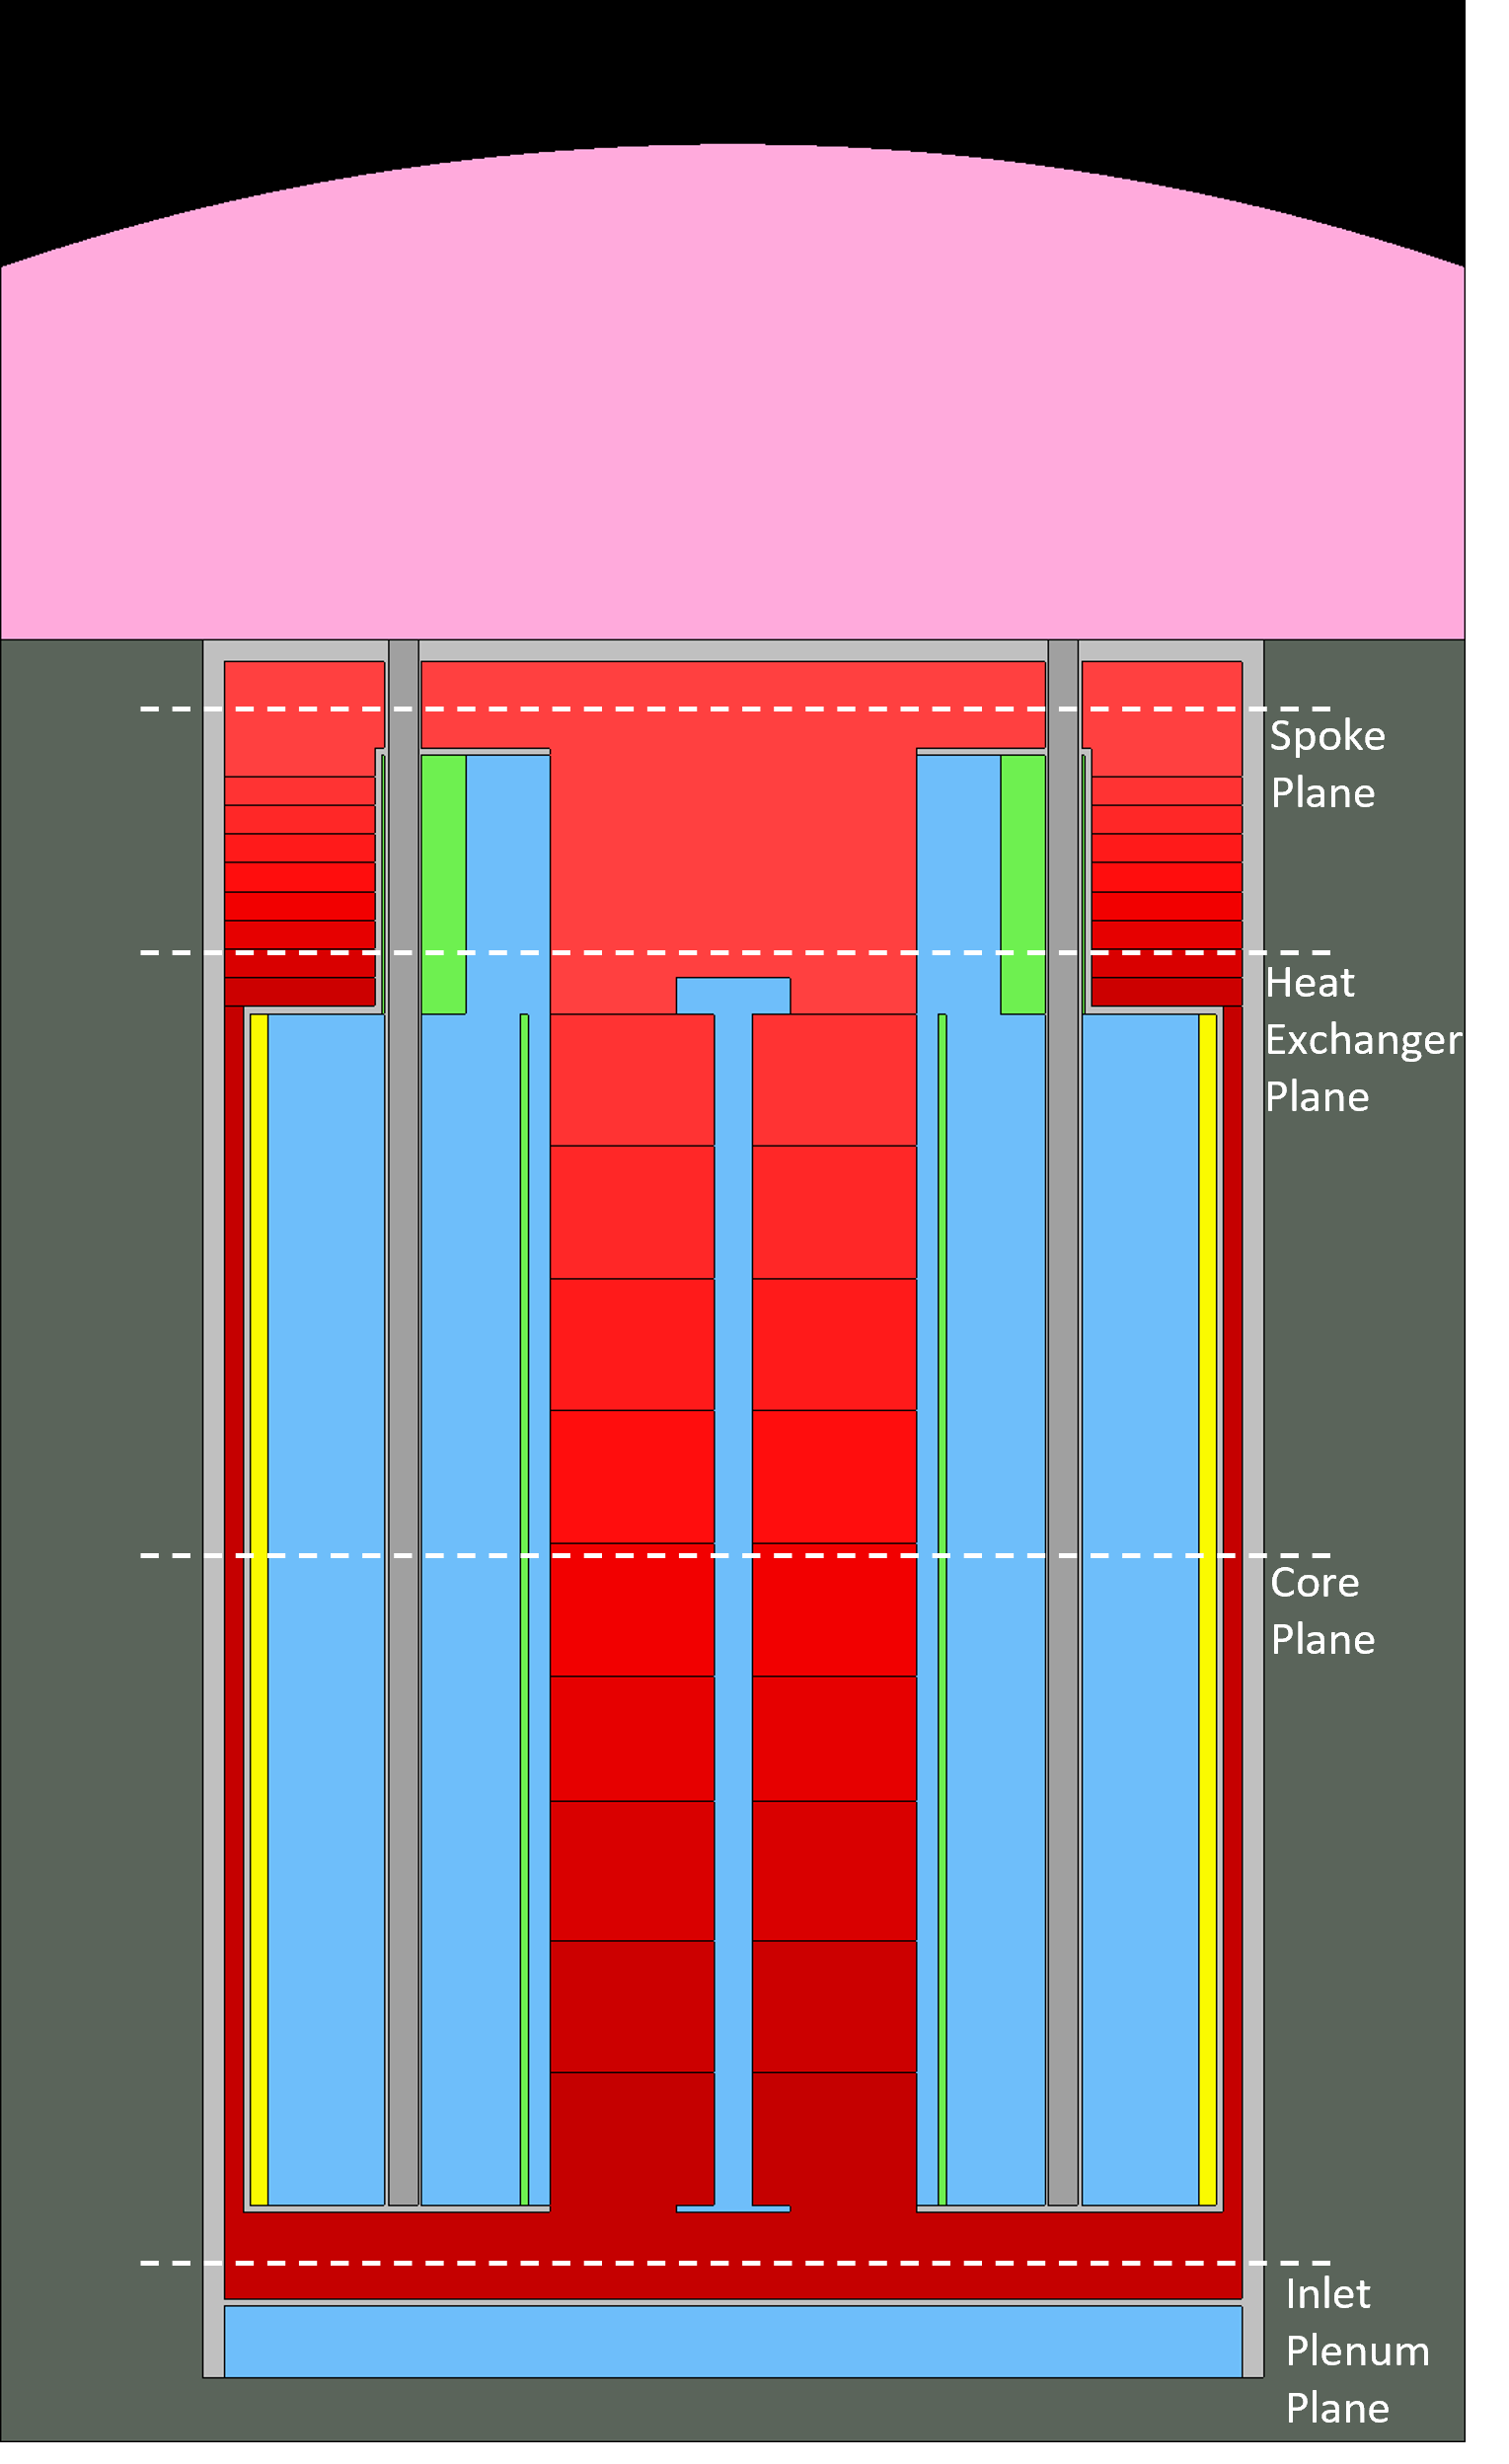
\includegraphics[width=0.75\textwidth]{Plotter/yz.png}
    \caption[Y-Z view of \acs{msnb}]{Y-Z view of \acs{msnb}. Molten salt is shown in red, with darker shades corresponding to a lower temperature and higher density. The core is surrounded by the beryllium-oxide reflector (blue) and the boron-carbide absorber plate (green). The core is separated from the riser by a a perforated reflector plate and the riser is separated from the heat exchanger by an absorbing ring. From this angle the internal moderating structure appears as only the center rod, as the fins exist in other planes.The cross-sectional planes plotted in Figure \ref{fig:Plotter-XY} are sketched.}
    \label{fig:Plotter-YZ}
\end{figure}
\clearpage
\begin{figure}[!ht]
    \centering
    \subfloat[\centering Inlet Plenum]{
\includegraphics[width=0.49\textwidth]{Plotter/inlet}}
    \subfloat[\centering Core]{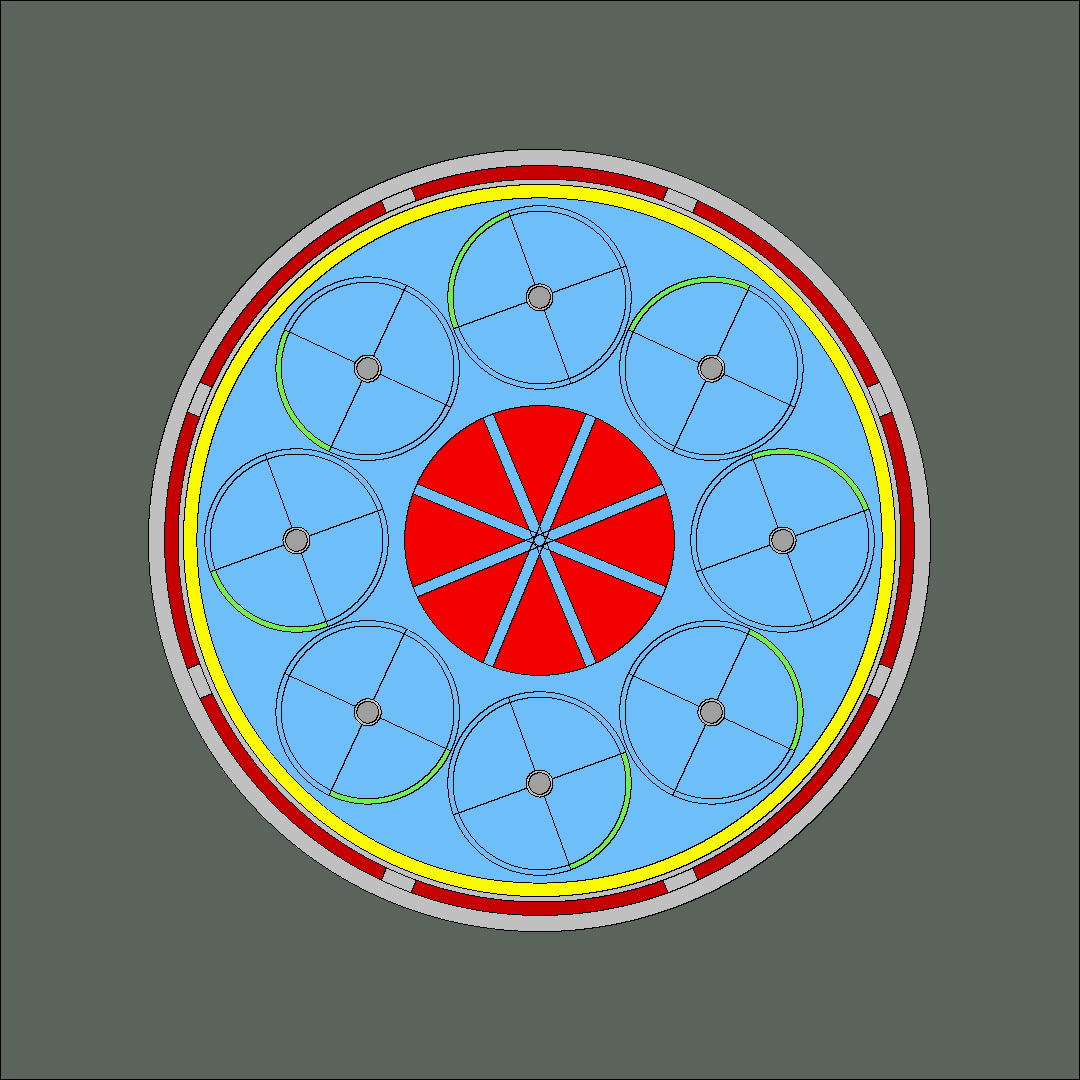
\includegraphics[width=0.49\textwidth]{Plotter/core}}
    \quad
    \subfloat[\centering Heat Exchanger]{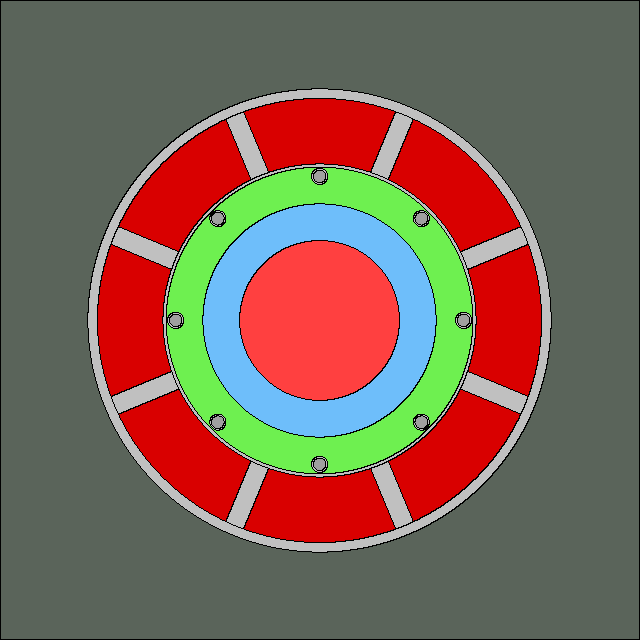
\includegraphics[width=0.49\textwidth]{Plotter/hex}}
    \subfloat[\centering Spoke]{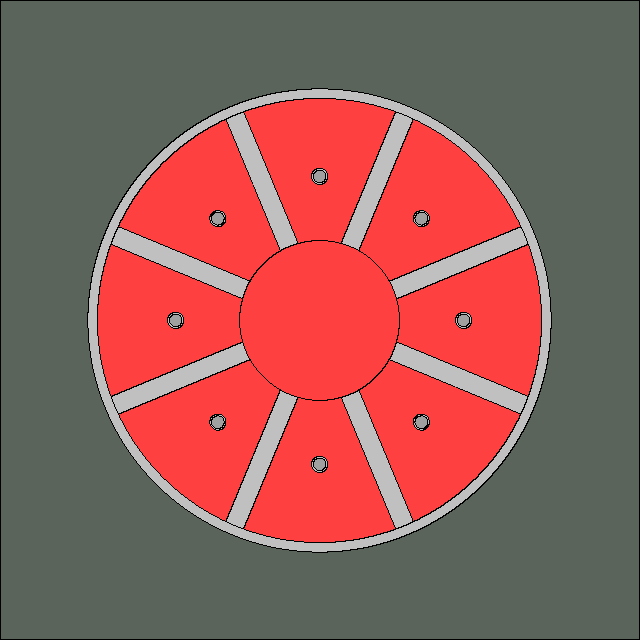
\includegraphics[width=0.49\textwidth]{Plotter/spoke}}
    \caption[X-Y Views of \acs{msnb}]{X-Y Views of \acs{msnb}
    \begin{enumerate*}[label=\alph*)]
        \item The inlet plenum sits below the downcomer, core, and reflector. Molten salt exiting the downcomer travels from the outer edge inward inward to the center, where it rises (out of the page) to enter the core;
        \item The core is surrounded by the reflector and control drums, which may be adjusted to manipulate criticality. The reflector and downcomer are separated by a graphite shield;
        \item The molten salt in the outer ring is in the heat exchanger. As it sinks (into the), heat is being rejected to the secondary coolant (not modeled). A ring of boron-carbide ensures that delayed neutrons emitted in the riser do not transport to the heat exchanger; 
        \item The spoke sits above the downcomer, core, and reflector.Molten salt exiting the riser travels radially outward to the top of the heat exchanger;
    \end{enumerate*}}
    \label{fig:Plotter-XY}
\end{figure}

\begin{figure}[!ht]
    \centering
    \subfloat[\centering Least Reactive]{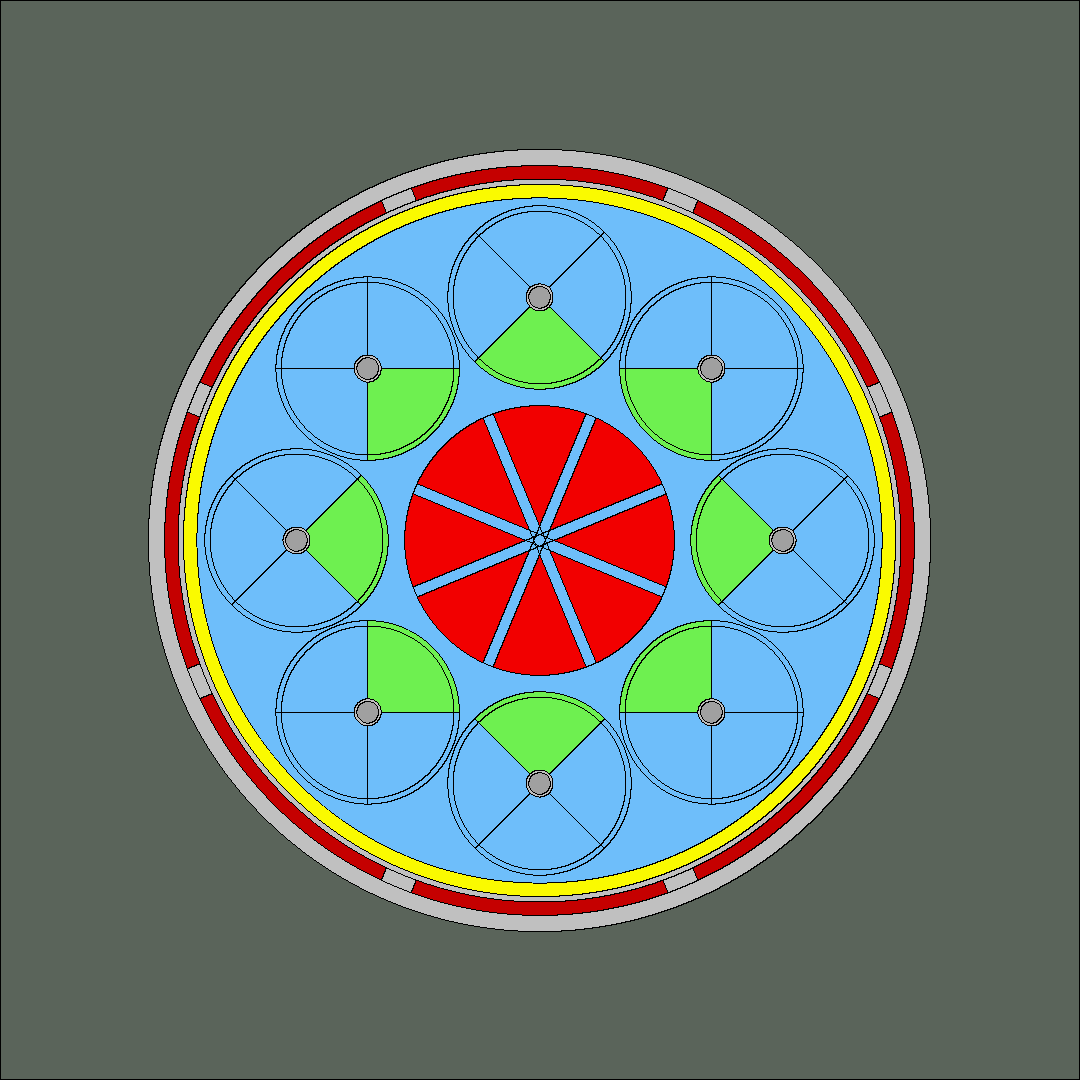
\includegraphics[width=0.33\textwidth]{Plotter/least.png}}
    \subfloat[\centering Initial Criticality]{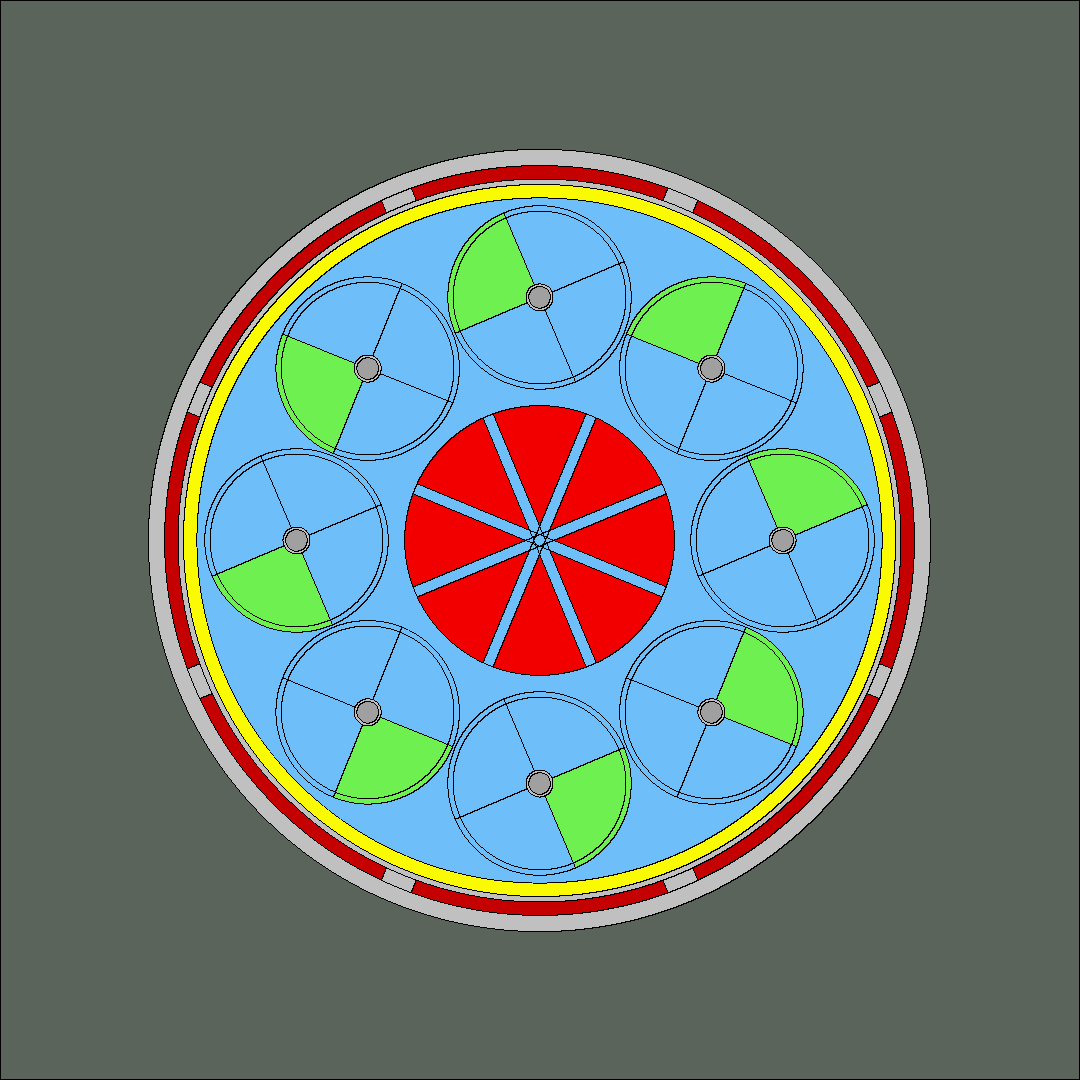
\includegraphics[width=0.33\textwidth]{Plotter/initial.png}}
    \subfloat[\centering Most Reactive]{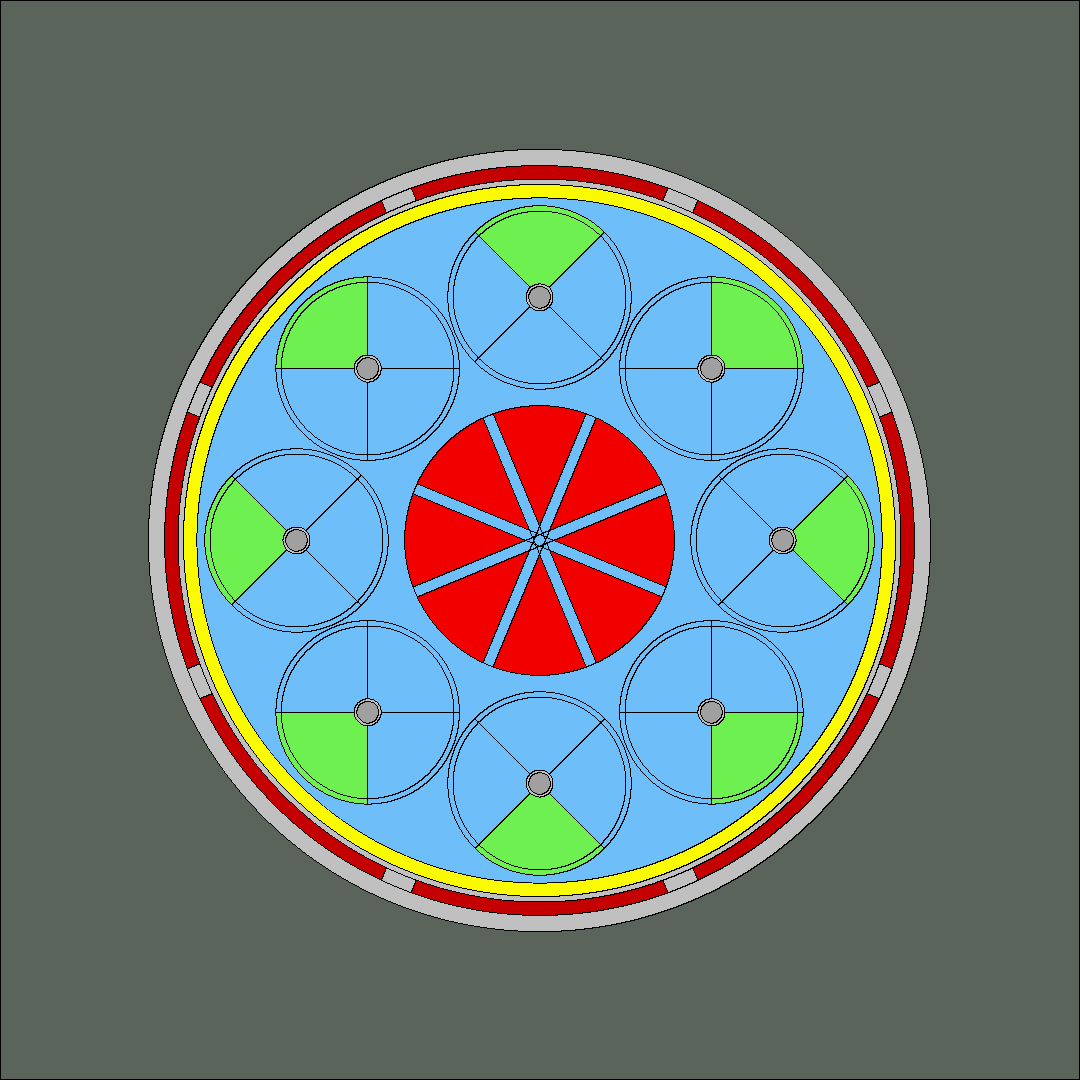
\includegraphics[width=0.33\textwidth]{Plotter/most}}
    \caption[X-Y View of \acs{msnb} - Control Drums]{X-Y Views of \acs{msnb} with control drums in three orientations:
    \begin{enumerate*}[label=\alph*)]
        \item 0 degrees, which is used to test the reactor's shutdown margin;
        \item 112 degrees, which is the initial critical orientation; and 
        \item 180 degrees, which is used to test the reactor's excess reactivity; 
    \end{enumerate*}
    Beryllium oxide is depicted in blue while boron carbide is green. The entire wedge of each control drum is colored for clarity. Only the outer rim is actually made from boron carbide.}
    \label{fig:Plotter-CD}
\end{figure}



\begin{figure}[!ht]
    \centering
    \resizebox{\textwidth}{!}{
\begin{tikzpicture}
    %Pre-filter
    \draw[->] (-6,0)node[anchor=east]{$\dot{Q}_{HEX}$} -- (-4.5,0);
    \draw (-4.5,-0.5) rectangle (-3.5,0.5) node[pos=0.5]{$F(s)$};
    %Sum
    \draw[->] (-3.5,0) -- (-2,0) node[pos=0.5,anchor=south]{$\dot{Q}_{Core}^{SP}$};
    \draw (-1.75,0) circle (0.25) node{\scriptsize$\textbf{-}$};
    %Controller
    \draw[->] (-1.5,0) -- (-0.5,0)node[pos=0.5,anchor=south]{$e$};
    \draw (-0.5,-0.5) rectangle (0.5,0.5) node[pos=0.5]{$C(s)$};
    \draw[->] (0.5,0) -- (1.5,0) node[pos=0.5,anchor=south]{$u_{CD}$};
    %Actuator
    \draw (1.5,-0.5) rectangle (2.5,0.5) node[pos=0.5]{$A(s)$};
    \draw[->] (2.5,0) -- (3.5,0) node[pos=0.5,anchor=south]{$\rho_{CD}$};
    %Sum
    \draw (3.75,0) circle (0.25) node{\scriptsize$\textbf{+}$};
    %Process
    \draw[->] (4,0) -- (5,0) node[pos=0.5,anchor=south]{$\rho$};
    \draw (5,-0.5) rectangle (6,0.5) node[pos=0.5]{$P(s)$};
    \draw[->] (6,0) -- (8,0) node[anchor=west]{$\dot{Q}_{Core}$};
    %Transducer
    \draw[->] (7,0) -- (7,-1.5) -- (2.5,-1.5);
    \draw (1.5,-2) rectangle (2.5,-1) node[pos=0.5]{$H(s)$} ;
    \draw[->] (1.5,-1.5) -- (-1.75,-1.5) -- (-1.75,-0.25);
    %Passive Feedback
    %Core Feedback
    \draw[->] (7,0) -- (7,2.5);
    \draw (6.5,2.5) rectangle (7.5,3.5) node[pos=0.5]{$G_{C}(s)$};
    \draw[->] (6.5,3) -- (4.25,3);
    %HEX Feedback
    \draw[->] (-5,0) -- (-5,2.5);
    \draw (-4.5,2.5) rectangle (-5.5,3.5) node[pos=0.5]{$G_{H}(s)$};
    \draw[->] (-4.5,3) -- (3.25,3)node[pos=0.5,anchor=south]{$T_{cold}$};
    %Sum
    \draw (3.75,1.5) circle (0.25) node{\scriptsize$\textbf{+}$};
    \draw[->](3.75,1.25) -- (3.75,0.25);
    %TemperatureFeedback
    \draw (1.5,1) rectangle (2.5,2) node[pos=0.5]{$\alpha_T$};
    \draw[->] (2.5,1.5) -- (3.5,1.5) node[pos=0.5,anchor=south]{$\rho_{T}$};
    %FlowFeedback
    \draw (3.25,2.5) rectangle (4.25,3.5) node[pos=0.5]{$\alpha_F$};
    \draw[->] (3.75,2.5) -- (3.75,1.75) node[pos=0.5,anchor=west]{$\rho_{F}$};
    %Downcomer
    \draw[->] (0,3) -- (0,2);
    \draw (-0.5,1) rectangle (0.5,2) node[pos=0.5]{$\theta_{DC}$};
    \draw[->] (0.5,1.5) -- (1.5,1.5);
    %Riser
    \draw[->] (5.375,3) -- (5.375,4.5) -- (0.5,4.5) node[pos=0.5,anchor=south]{$T_{hot}$};
    \draw (-0.5,4) rectangle (0.5,5) node[pos=0.5]{$\theta_{R}$};
    \draw[->] (-0.5,4.5) -- (-5,4.5) -- (-5,3.5);


\end{tikzpicture}
}
    \caption[Control loop of a natural circulation \acs{msnb}]{Control loop of a natural circulation \acs{msnb}. It is a normal feedback loop with a pre-filter, with the addition of the passive feedback mechanisms. The core ($\dot{Q}_{Core}$) and heat exchanger ($\dot{Q}_{HEX}$) powers go through the respective temperature dynamics ($G_C$ and $G_H$) and time delays for the riser ($\theta_R$) and downcomer ($\theta_{DC}$) before being converted to reactivity by the temperature($\alpha_T$) and flow ($\alpha_F$) feedback mechanisms. The passive reactivity feedback is combined with the control drum reactivity ($\rho_{CD}$) and fed into the reactor dynamics ($P(s)$).  }
    \label{fig:ReactorControlLoop}
\end{figure}

\begin{figure}[ht!]
    \centering
    \resizebox{0.5\textwidth}{!}{\begin{tikzpicture}
    %blocks
    \draw (-2,-0.5) rectangle (-1,0.5) node[pos=0.5]{NC};
    \draw (1,-0.5) rectangle (2,0.5) node[pos=0.5]{RPK};
    \draw (-0.5,1.9) rectangle (0.5,2.9) node[pos=0.5]{USUF};
    
    %inner arrows
    \draw[->] (0,1.9) -- (0,0.85);
    \draw node at (0,0.7) {\tiny Temp-Profile};
    \draw[->] (-0.2,0.55) -- (-0.95,0);
    \draw[->] (0.2,0.55) -- (0.95,0);

    %outer arrows
    \draw[->] (-1.75,0.5) arc (180:112.5:2) node[midway,sloped,above]{\tiny Flow Rate};
    \draw[->] (-1.5,-0.5) arc (225:315:2) node[midway,sloped,below]{\tiny Flow Rate};
    \draw[->] (1.75,0.5) arc (0:67.5:2) node[midway,sloped,above]{\tiny Core Power};
\end{tikzpicture}}
    \caption[Process simulator logic flow diagram]{\raggedright Logic flow diagram for the \acs{msnb} transient process simulator.}
    \label{fig:PythonFlowDiagram}
\end{figure}




\newpage



%\begin{appendices}


%%%%% use for toc
%    \titleformat{\part}{\normalfont\Large\bfseries\filcenter}{\thepart}{0ex}{}[]
%    \part*{Appendices}
%%%%%


%    \setcounter{section}{0}
%    \renewcommand{\thesection}{\Roman{section}}
%    \titleformat{\section}{\normalfont\large\bfseries}{Appendix \thesection:}{1ex}{}[]


%    \section{Just appendix title} \label{app-}


%\end{appendices}


\end{document}